\label{Cocomo}
Cocomo ist eine Anwendung zur Aufwandseinschätzung in der Softwareentwicklung. Dahinter steckt ein mathematisches Modell, welches mit Hilfe einer Vielzahl von  Parametern eine Kostenschätzung, sowohl in zeitlicher, als auch in monetärer Hinsicht, erstellt. Gerechnet wird in Personenmonaten oder Personenjahren, um diese möglichst genau angeben zu können sind die meisten gewünschten Parameter sehr firmen- und projektspezifisch. Die Basis für das Ergebnis der Einschätzung sind die im Projekt erwarteten Codezeilen, wobei man zwischen tatsächlich abgegebenem Code an den Kunden und dem gesamten Projekt inklusive der Testsoftware unterscheidet. Ist die Anzahl der benötigten Codezeilen bestimmt geht man über zur Komplexitätseinschätzung. Diese stellt drei Schwierigkeitsstufen zur Verfügung, organic mode, semi-detached und embedded. Dies sind nur beispielhafte oberflächliche Einstellungen, wie sie in diesem Projekt zur Aufwandseinschätzung 
verwendet wurden. \\ \\
% Screenshot von Cocomo einbinden
% mit sinnvoller Caption... (Unten ist auskommentiert die Vorlage zur Screenshotimplementierung)
% passender Text dazu noch schreiben
% bis Sonntag 19. April fertig machen!!!

\begin{figure}[!hbt]
	\centering
	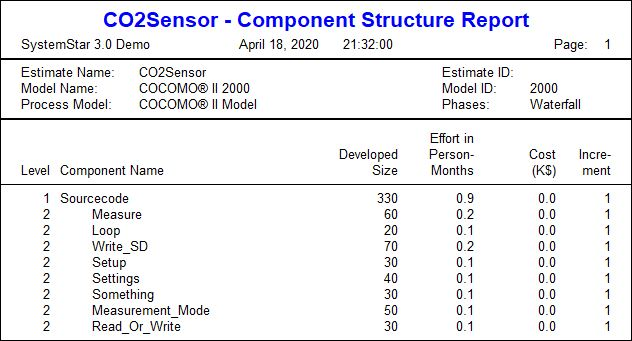
\includegraphics[width=0.9\linewidth]{Images/CocomoSchaetzung}
	\caption{Lines of Code Schätzung}
	\label{fig:Cocomo}
\end{figure}

Zuerst wurden die Anzahl der Codezeilen für jede einzelne Funktion eingeschätzt, die später auch im Endprodukt stehen sollten. Dabei ergaben sich 330 Zeilen Programmcode, welche laut \ref{Cocomo} in 0,9 Personenmonaten abgearbeitet werden fertiggestellt sind. Die monetären Kosten hierfür belaufen sich auf 0€, da dies eine Projektarbeit ist und somit keine Bezahlung erfolgt.